%%%%%%%%%%%%%%%%%%%%%%%%%%%%%%%%%%%%%%%%%%%%%%%%%%%%%%%%%%%%%%%%%%%%%%%%%%%%%%%%
% ICC-12 (2026) submission -- reconciled to the accompanying ugv_uav_control
% codebase. Claims are tagged so that PROVEN(offline)/IMPLEMENTED/SIMULATED/
% FUTURE are never blurred. See Sec. VI (Theoretical Properties &
% Implementation Status) and the claim-status table.
%%%%%%%%%%%%%%%%%%%%%%%%%%%%%%%%%%%%%%%%%%%%%%%%%%%%%%%%%%%%%%%%%%%%%%%%%%%%%%%%

\documentclass[letterpaper, 10 pt, conference]{ieeeconf}  % Comment this line out if you need a4paper

%\documentclass[a4paper, 10pt, conference]{ieeeconf}      % Use this line for a4 paper
\usepackage{amsmath}
\usepackage{amssymb}
\usepackage{graphicx}
% Figures resolve locally from the repo root (via the path below) and on Overleaf
% when the figure files are uploaded flat to the project root (bare filenames).
\graphicspath{{03_System_Integration_ROS2/results/}{./}}
\usepackage{tikz}
\usetikzlibrary{arrows.meta,positioning,calc,fit,backgrounds}

\IEEEoverridecommandlockouts                              % This command is only needed if
                                                          % you want to use the \thanks command

\overrideIEEEmargins                                      % Needed to meet printer requirements.

% ---- claim-status tags: keep proven/implemented/sim/future explicit ----
\newcommand{\tagOFFLINE}{{\footnotesize\textsc{[proven-offline]}}}
\newcommand{\tagIMPL}{{\footnotesize\textsc{[implemented]}}}
\newcommand{\tagSIM}{{\footnotesize\textsc{[simulation]}}}
\newcommand{\tagFUTURE}{{\footnotesize\textsc{[future work]}}}
\DeclareMathOperator{\tr}{tr}
\newcommand{\Rset}{\mathbb{R}}

% ---- results macros: computed by scripts/fill_paper_numbers.py from fresh logs; all
%  values also emitted to results/Table_1_Summary.csv (table and prose share one window).
%  STEADY-STATE window t>=8s (skip takeoff/EKF-convergence transient) for tracking error
%  and mean cov; peak cov reported BOTH full-run (transient-dominated) and over the
%  injected [20,28]s EKF-block window. R=4 repeats x {nominal,occlusion}=8 runs/method.
\newcommand{\RESsolvesCone}{331$\pm$3}\newcommand{\RESsolvesCthree}{29$\pm$1}
\newcommand{\RESerrCone}{0.065$\pm$0.001}\newcommand{\RESerrCthree}{0.064$\pm$0.001}
\newcommand{\REScovCone}{0.0148$\pm$0.0084}\newcommand{\REScovCthree}{0.0148$\pm$0.0084}
\newcommand{\RESpeakCone}{0.168$\pm$0.001}\newcommand{\RESpeakCthree}{0.170$\pm$0.001}
\newcommand{\RESpeakfullCone}{0.245$\pm$0.161}\newcommand{\RESpeakfullCthree}{0.197$\pm$0.166}
\newcommand{\RESaruCone}{6.2$\pm$0.2}\newcommand{\RESaruCthree}{9.0$\pm$0.2}

\title{\LARGE \bf
An Event-Triggered Tube-MPC Framework for Aerial--Ground Tracking: \\
Design and Computational Evaluation
}

\author{Shlok Mehndiratta$^{1}$, Divyam Sood$^{1}$, and Prashant Gupta$^{1}$%
\thanks{*This work was carried out as part of the LCS-334 Linear Control Systems project.}%
\thanks{$^{1}$The authors are with the Indian Institute of Science Education and
Research (IISER) Bhopal, India.
{\tt\small \{shlokm23, divyam23, prashant23\}@iiserb.ac.in}}%
}


\begin{document}



\maketitle
\thispagestyle{empty}
\pagestyle{empty}


%%%%%%%%%%%%%%%%%%%%%%%%%%%%%%%%%%%%%%%%%%%%%%%%%%%%%%%%%%%%%%%%%%%%%%%%%%%%%%%%
\begin{abstract}
We present an event-triggered tube-MPC framework for aerial--ground cooperative
tracking, integrated end-to-end in ROS\,2/Gazebo (software-in-the-loop), whose
perception-driven trigger reduces online planner solves by $\approx\!11\times$ at
statistically equal tracking accuracy in our evaluation. A quadrotor UAV
(abstracted as a velocity-controlled point mass) is the sole exteroceptive sensor
for a unicycle UGV observed through a downward camera and an ArUco marker. The design couples
perception and control through four implemented components: (i) a belief-space
nonlinear MPC for the UGV that propagates the EKF covariance through its horizon
and penalizes predicted covariance trace and field-of-view (FoV) exit; (ii) an
ancillary tube regulator for the UAV that uses an ellipsoidal invariant-set bound
whose radius scales with the EKF covariance; (iii) a multi-condition event trigger
that replans on tube exit, covariance spikes, anticipated path curvature, or
temporal drift; and (iv) a view-quality-dependent EKF measurement model. A minimal
robust positively invariant (mRPI) set is derived offline as a certified robust
bound but is \emph{not} wired into the online loop, which uses the ellipsoidal
bound of (ii). Our validated quantitative result is \emph{computational}: across
$8$ paired runs the event trigger reduces online planner solves by $\approx\!11\times$
($331\pm3\to29\pm1$ per run) at statistically indistinguishable tracking error.
The trigger is observability-aware \emph{by design}; we claim only this compute
payoff, and we document (Sec.~\ref{sec:theory}) why an isolated observability
benefit of the trigger is not demonstrable on the present platform. Throughout we
mark which properties are proven offline, implemented, shown in simulation, or
future work.
\end{abstract}


%%%%%%%%%%%%%%%%%%%%%%%%%%%%%%%%%%%%%%%%%%%%%%%%%%%%%%%%%%%%%%%%%%%%%%%%%%%%%%%%
\section{INTRODUCTION}

The deployment of Unmanned Ground Vehicles (UGVs) in unstructured and GPS-denied
environments is heavily constrained by their limited perception horizons.
Ground-level sensors such as LiDAR and stereo cameras suffer from occlusion,
narrow fields of view (FoV), and an inability to anticipate upcoming path
curvature. To mitigate this, aerial--ground cooperative systems employ an
Unmanned Aerial Vehicle (UAV) as an elevated ``eye in the sky'' for a
perception-limited UGV.

Most cooperative-tracking frameworks treat the UAV as a \emph{passive} observer:
it follows a predefined trajectory or simply minimizes distance to the UGV,
treating the UGV's state estimation as a downstream byproduct
\cite{mayne2000constrained}. This decoupling is fragile: when the UGV maneuvers
aggressively or is occluded, the UAV can lose the target, the estimation
covariance grows, and tracking degrades. Active-perception planning, where the
sensor trajectory is optimized to maximize information gain
\cite{falanga2018pampc}, addresses part of this but typically relies on
continuous, computationally expensive replanning and rarely integrates robust
tracking guarantees for the aerial vehicle.

This paper studies a \emph{bidirectional} observability-aware architecture in
which \emph{both} vehicles adapt to the ground vehicle's estimation uncertainty.
Its contributions, as realized in the accompanying open implementation, are:

\begin{itemize}
\item \textbf{An observability-driven event-triggered tube-MPC design} integrating a
covariance/FoV-penalizing belief-space UGV controller
\cite{platt2010belief,vandenberg2012motion}, a covariance-scaled ellipsoidal tube
regulator \cite{mayne2005robust} (with an offline-certified mRPI bound
\cite{mRPI}), and a multi-condition perception trigger \cite{eqtami2010event} on
tube exit, covariance spikes, anticipated curvature, or temporal drift. The
covariance-scaling and FoV terms are design properties; we do \emph{not} claim they
are shown to improve observability (Sec.~\ref{sec:theory}). \tagIMPL

\item \textbf{A full SITL integration} in ROS\,2/Gazebo --- vision/ArUco pipeline,
view-quality-coupled EKF, and coupled UGV/UAV controllers --- demonstrated to run
the design end-to-end; integration alone does not evidence efficacy of the coupling. \tagIMPL

\item \textbf{A validated computational result}: the perception-driven trigger cuts
online planner solves by $\approx\!11\times$ at equal tracking accuracy (reproducible
$6$\,m regime, $8$ paired runs). This solve-count reduction is the validated payoff;
the observability benefit of the covariance scaling is \emph{not} isolated
(Sec.~\ref{sec:theory}). \tagSIM
\end{itemize}
The trigger's \emph{design} is observability-aware; its \emph{demonstrated} payoff
is computational. We keep these separate throughout, and Sec.~\ref{sec:theory}
states precisely why the isolated observability benefit is not testable at the
present scope.

We deliberately separate the idealized robust-MPC theory (offline mRPI, tightened
constraints, terminal-set recursive feasibility) from what the code enforces
online, and we validate the computational claim in simulation. The remainder of
the paper is organized as follows. Section~\ref{sec:related} reviews related
work; Section~\ref{sec:problem} states the problem; Section~\ref{sec:arch} gives
the vehicle and perception models; Section~\ref{sec:method} develops the coupled
event-triggered tube-MPC; Section~\ref{sec:theory} states the theoretical
properties and the exact implementation status; and Section~\ref{sec:results}
reports the simulation study.

\section{RELATED WORK}
\label{sec:related}

\textbf{Robust and tube MPC.} Tube MPC \cite{mayne2005robust} decomposes control
into a nominal plan and an ancillary law that confines the true state to a robust
positively invariant (RPI) tube; Rakovi\'c et al. \cite{mRPI} give the standard
outer approximation of the minimal RPI set by a truncated Minkowski series. These
guarantees assume a fixed, bounded disturbance set and constraint tightening
computed offline. Time-varying (homothetic/parameterized) tubes generalize the
fixed tube but require the scaling to enter the optimization with its own
feasibility argument; our online adaptivity (Section~\ref{sec:method}) is a
lighter-weight surrogate and we mark the homothetic treatment as future work.

\textbf{Perception-aware and active planning.} PAMPC \cite{falanga2018pampc}
optimizes quadrotor trajectories for perception objectives. Belief-space planning
\cite{platt2010belief,vandenberg2012motion} augments the planning state with the
estimator covariance. Our belief-space UGV controller is in this family. The
\emph{bidirectional} coupling --- the \emph{target} shaping its trajectory to stay
observable while the \emph{tracker} adapts its robustness to perception quality ---
is the design novelty of the architecture. What we \emph{evidence} in this paper is
narrower and concrete: the integrated SITL realization of that architecture and the
perception-driven trigger's computational result (Sec.~\ref{sec:results}).
Isolating the coupling's observability benefit is future work requiring a
controllable-lag, trajectory-reproducible regime (Sec.~\ref{sec:theory}).

\textbf{Event-triggered MPC.} Event-triggered schemes \cite{eqtami2010event}
re-solve only when a state-dependent condition fires. We instantiate a
perception-driven trigger with a critical tube-exit condition plus anticipatory
conditions.

\section{PROBLEM FORMULATION}
\label{sec:problem}

A UAV tracks a UGV in a global frame $\mathcal{F}_W$. The UAV carries the only
exteroceptive sensor: a downward monocular camera that detects an ArUco marker on
the UGV, yielding a noisy pose measurement whose quality depends on the imaging
geometry. An EKF fuses these detections with UGV wheel odometry to produce a
belief $(\mu,\Sigma)$ over the UGV state. The objective is to (i) keep the UGV
inside the camera footprint so that $\Sigma$ stays bounded, (ii) track the UGV
robustly under bounded disturbances, and (iii) do so while limiting the number of
online optimizations. The UGV must track a ground lane while remaining
observable.

\section{System Architecture and Models}
\label{sec:arch}

Fig.~\ref{fig:system} shows the implemented system and its signal flow.

\begin{figure}[t]
\centering
\resizebox{0.99\columnwidth}{!}{%
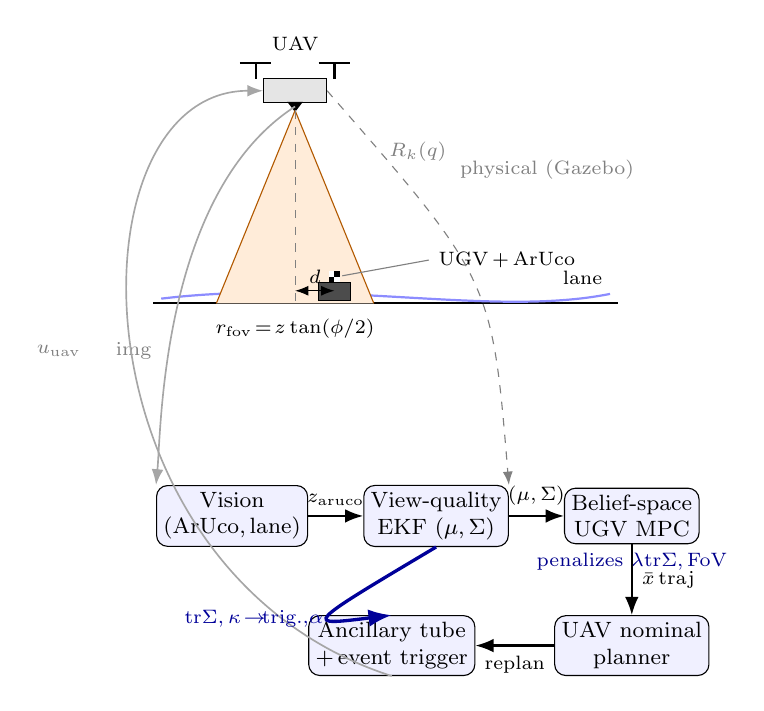
\begin{tikzpicture}[font=\footnotesize,>=Latex,
  blk/.style={draw,rounded corners,align=center,minimum height=6.5mm,inner sep=2.5pt,fill=blue!6},
  sig/.style={->,thick},
  loop/.style={->,semithick,gray!70},
  cpl/.style={->,very thick,blue!60!black},
  faint/.style={->,dashed,gray}]
% physical scene
\draw[thick] (-0.3,0) -- (5.6,0);
\draw[thick,blue!45] (-0.2,0.06) .. controls (2,0.32) and (4,-0.18) .. (5.5,0.12);
\node at (5.15,0.32) {\scriptsize lane};
\node[draw,fill=gray!20,minimum width=8mm,minimum height=3mm] (uavbody) at (1.5,2.7) {};
\draw[thick] (1.0,2.85)--(1.0,3.05) (2.0,2.85)--(2.0,3.05);
\draw[thick] (0.8,3.05)--(1.2,3.05) (1.8,3.05)--(2.2,3.05);
\node at (1.5,3.3) {\scriptsize UAV};
\coordinate (cam) at (1.5,2.5);
\fill[black] (1.4,2.56)--(1.6,2.56)--(1.5,2.43)--cycle;
\fill[orange!15] (1.5,2.45) -- (0.5,0) -- (2.5,0) -- cycle;
\draw[orange!70!black] (1.5,2.45)--(0.5,0);\draw[orange!70!black] (1.5,2.45)--(2.5,0);
\draw[dashed,gray] (1.5,2.45)--(1.5,0);
\draw[|<->|] (0.5,-0.32)--(2.5,-0.32) node[midway,fill=white,inner sep=1pt]{\scriptsize $r_{\mathrm{fov}}\!=\!z\tan(\phi/2)$};
\node[draw,fill=black!70,minimum width=4mm,minimum height=2.2mm] (ugv) at (2.0,0.15) {};
\fill[black] (1.93,0.27) rectangle (2.07,0.41);
\fill[white] (1.93,0.34) rectangle (2.0,0.41);\fill[white] (2.0,0.27) rectangle (2.07,0.34);
\node[anchor=west] at (3.2,0.55) (ugvlab) {\scriptsize UGV\,+\,ArUco};
\draw[gray] (ugvlab.west)--(2.1,0.35);
\draw[<->] (1.5,0.16)--(2.0,0.16); \node at (1.75,0.34){\scriptsize $d$};
\node[gray] at (4.7,1.7){\scriptsize physical (Gazebo)};
% blocks
\node[blk] (vis) at (0.7,-2.7) {Vision\\(ArUco,\,lane)};
\node[blk,right=7mm of vis] (ekf) {View-quality\\EKF $(\mu,\Sigma)$};
\node[blk,right=7mm of ekf] (ugvmpc) {Belief-space\\UGV MPC};
\node[blk,below=9mm of ugvmpc] (plan) {UAV nominal\\planner};
\node[blk,left=10mm of plan] (anc) {Ancillary tube\\+\,event trigger};
\node[blue!55!black,font=\scriptsize,align=center,below=0.5pt of ugvmpc.south,yshift=1pt]{penalizes $\lambda\mathrm{tr}\Sigma$,\,FoV};
% forward flow
\draw[loop] (cam) .. controls (-0.2,1.4) and (-0.2,-1.6) .. (vis.north west); \node[gray] at (-0.55,-0.6){\scriptsize img};
\draw[sig] (vis) -- node[above]{\scriptsize $z_{\mathrm{aruco}}$} (ekf);
\draw[sig] (ekf) -- node[above]{\scriptsize $(\mu,\Sigma)$} (ugvmpc);
\draw[sig] (ugvmpc) -- node[right]{\scriptsize $\bar{x}$\,traj} (plan);
\draw[sig] (plan) -- node[below]{\scriptsize replan} (anc);
\draw[loop] (anc.south) .. controls (-1.4,-3.4) and (-1.4,2.7) .. (uavbody.west);
\node[gray] at (-1.5,-0.6){\scriptsize $u_{\mathrm{uav}}$};
% coupling (b)
\draw[cpl] (ekf.south) .. controls (1.6,-4.1) .. (anc.north) node[pos=0.62,left=-1pt]{\scriptsize $\mathrm{tr}\Sigma,\kappa\!\to\!$trig.,$\alpha$};
\draw[faint] (uavbody.east) .. controls (4.0,0.3) .. (ekf.north east) node[pos=0.12,right]{\scriptsize $R_k(q)$};
\end{tikzpicture}}
\caption{Implemented system and signal flow. A downward-camera UAV (footprint
radius $r_{\mathrm{fov}}=z\tan(\phi/2)$) observes an ArUco-tagged UGV at horizontal
offset $d$. \textbf{Black:} forward data flow (vision$\to$EKF$\to$belief-space UGV
MPC$\to$UAV nominal planner$\to$ancillary tube/event trigger$\to$UAV);
\textbf{blue:} the perception$\to$control couplings actually used --- the UGV cost
penalizes $\lambda\,\mathrm{tr}\Sigma$ and FoV exit, and the EKF covariance/curvature
drive the event trigger and tube radius $\alpha$; \textbf{dashed grey:} the modeled
dependence of measurement noise $R_k(q)$ on UAV geometry. All arrows are implemented
ROS\,2 signals; the figure asserts no performance claim.}
\label{fig:system}
\end{figure}

\subsection{UGV dynamics}
The UGV uses unicycle kinematics with first-order actuator lag. Let
$\mathbf{x}_g = [x_g, y_g, \theta, v, \omega]^T$ be the state, $(x_g,y_g)$ the
position, $\theta$ the heading, $(v,\omega)$ the linear/angular velocities, and
$\mathbf{u}_g = [v_c, \omega_c]^T$ the commanded velocities. The discrete-time
dynamics are
\begin{equation}
\mathbf{x}_{g,k+1} = \mathbf{f}_g(\mathbf{x}_{g,k}, \mathbf{u}_{g,k}) + \mathbf{w}_g,
\end{equation}
where the actuator lag is governed by time constants $\tau_v,\tau_\omega$ and
$\mathbf{w}_g$ is process noise. \tagIMPL

\subsection{UAV model}
Although the platform is a quadrotor, the planner and the ancillary tracker treat
it as a \textbf{velocity-controlled point mass} (single integrator); an
inner-loop attitude/thrust controller, provided by the Gazebo velocity-control
plugin, is assumed to realize commanded velocities. With position
$\mathbf{p}=[p_x,p_y,p_z]^T$ and velocity command $\mathbf{u}=[v_x,v_y,v_z]^T$,
\begin{equation}
\mathbf{p}_{k+1} = \mathbf{p}_k + \Delta t\, \mathbf{u}_k + \mathbf{w}_k,
\qquad A_d=I_3,\ B_d=\Delta t\, I_3,
\label{eq:uav_disc}
\end{equation}
with bounded disturbance $\mathbf{w}_k\in\mathbb{W}$. Vertical velocity is a
genuine decision variable, so altitude is planned rather than fixed. A
second-order double-integrator (acceleration input) is the more faithful
rigid-body abstraction; we use \eqref{eq:uav_disc} because it is exactly what the
implementation optimizes. \tagIMPL

\subsection{View-quality-dependent perception}
The camera's vantage point affects estimation accuracy. We use a differentiable
view-quality metric $q_k\in(0,1]$ that degrades as the UGV nears the FoV edge and
as the altitude departs from a precision-optimal value $z_{\mathrm{opt}}$ (too low
loses footprint; too high loses pixel resolution). With horizontal UAV--UGV
distance $d=\lVert\mathbf{p}^{xy}-\mathbf{p}_g\rVert$ and footprint radius
$r_{\mathrm{fov}}(z)=z\tan(\phi/2)$,
\begin{equation}
q_k =
\underbrace{\frac{1}{1+e^{\beta(d-r_{\mathrm{fov}})}}}_{\text{FoV gate}}\!\cdot\!
\underbrace{e^{-d^2/(2\sigma_{xy}^2)}}_{\text{centering}}\!\cdot\!
\underbrace{e^{-(z-z_{\mathrm{opt}})^2/(2\sigma_z^2)}}_{\text{altitude precision}},
\label{eq:q}
\end{equation}
with $\sigma_{xy}=r_{\mathrm{fov}}/2$. The altitude factor makes $q_k$
\emph{non-monotone} in $z$ (it does not tend to $1$ as $z\to\infty$), removing the
incentive to climb without bound. \tagIMPL

The measurement covariance grows as view quality drops. The implementation scales
the baseline ArUco covariance $R_{\mathrm{full}}$ inversely with $q_k$,
\begin{equation}
R_k(q_k) = \frac{R_{\mathrm{full}}}{q_k + \epsilon},
\qquad \epsilon=10^{-3},
\label{eq:Rk}
\end{equation}
so $R_k\to R_{\mathrm{full}}$ for an excellent view and $R_k\to\infty$ (the
update ignores the marker) as $q_k\to0$. This couples UAV geometry directly to
EKF performance. \tagIMPL

\section{Coupled Event-Triggered Tube MPC}
\label{sec:method}

The estimation uncertainty $\Sigma_k$ enters the control formulations of both
vehicles.

\subsection{Information-aware UGV control (belief-space NMPC)}
The UGV controller augments the planning state with the covariance,
$\xi_k=(\mu_k,\Sigma_k)$, and \emph{propagates both through the horizon}. At each
predicted step it forms the no-observation prediction
$\Sigma_{\mathrm{pred}}=F\Sigma F^T+Q$ and a post-measurement covariance
$\Sigma_{\mathrm{obs}}$ (Joseph update with $R_k$ from \eqref{eq:Rk}), and blends
them by a smooth visibility gate
$\gamma=1/(1+e^{\beta(d-r_{\mathrm{fov}})})$:
\begin{equation}
\Sigma_k = (1-\gamma)\,\Sigma_{\mathrm{pred}} + \gamma\,\Sigma_{\mathrm{obs}}.
\label{eq:blend}
\end{equation}
The cost minimizes tracking error while penalizing predicted uncertainty and FoV
exit,
\begin{equation}
J_g = \sum_{k=0}^{N_g-1}\!\Big(
\lVert\mathbf{e}_{g,k}\rVert_Q^2
+\lVert\mathbf{u}_{g,k}\rVert_R^2
+\lambda\,\tr(\Sigma_k)
+ w_{\mathrm{fov}}\,c_{\mathrm{fov}}(\mathbf{x}_{g,k})\Big),
\label{eq:Jg}
\end{equation}
where the FoV term is a one-sided quadratic hinge
$c_{\mathrm{fov}}=\big(\max(0,\,d_k-r_{\mathrm{fov}})\big)^2$ (a soft constraint,
not an asymptotic barrier). The covariance rollout \eqref{eq:blend} makes
\eqref{eq:Jg} a nonconvex NLP, solved with SLSQP over $N_g=5$. The two terms
$\lambda\tr(\Sigma_k)$ and $w_{\mathrm{fov}}c_{\mathrm{fov}}$ are what make the
controller belief-coupled and are absent from the passive baseline. \tagIMPL

\subsection{Aerial nominal planner}
The UAV computes a nominal trajectory $\bar{\mathbf{p}}$ over $N_a=10$ by
optimizing goal tracking, an altitude regularizer toward $z_{\mathrm{opt}}$, and a
visibility term that tolerates lateral offset only when altitude is sufficient:
\begin{equation}
\begin{aligned}
J_a = \sum_{k}w_{\ell,k}\Big[\,
&\lVert\bar{\mathbf{p}}_k-\mathbf{g}\rVert^2
+ w_z(z_k-z_{\mathrm{opt}})^2 \\[-1pt]
&+ w_{\mathrm{alt}}\frac{\lVert\bar{\mathbf{p}}^{xy}_k-\mathbf{g}^{xy}\rVert^2}{z_k^2+0.1}
\,\Big] + w_u\lVert\bar{\mathbf{u}}_k\rVert^2,
\end{aligned}
\label{eq:Ja}
\end{equation}
where $\mathbf{g}$ is the UGV's predicted end-of-horizon position (read from the
belief-MPC rollout, one direction of the coupling) and $w_{\ell,k}$ up-weights
later steps. The weights are fixed (not re-scaled online); ``climb into turns to
widen the footprint'' is an emergent optimum of \eqref{eq:Ja}, not a hand-coded
rule. \tagIMPL

\subsection{Offline robust invariant set (tube) derivation}
\label{sec:mrpi}
The ancillary law is $\mathbf{u}_k=\bar{\mathbf{u}}_k-K\mathbf{e}_k$ with tracking
error $\mathbf{e}_k=\mathbf{p}_k-\bar{\mathbf{p}}_k$; substituting into
\eqref{eq:uav_disc},
\begin{equation}
\mathbf{e}_{k+1}=\underbrace{(A_d-B_dK)}_{=:A_K}\mathbf{e}_k+\mathbf{w}_k,
\qquad \mathbf{w}_k\in\mathbb{W}.
\label{eq:error_dynamics}
\end{equation}
Unlike standard tube MPC, we account for measurement noise $\mathbf{v}_k$ entering
through the feedback gain; the effective disturbance is
$\mathbf{w}_{\mathrm{eff}}=\mathbf{w}_a-B_dK\mathbf{v}_k$, and for the offline
computation $\mathbf{v}_k$ is bounded to a box (a hard, undocumented-confidence
truncation of the otherwise Gaussian noise; see Section~\ref{sec:theory}). For
$A_K$ Schur and $\mathbb{W}$ compact, the minimal RPI set is
$\Omega_\infty=\bigoplus_{i=0}^{\infty}A_K^i\mathbb{W}$, which we outer-approximate
by truncating after $N=100$ terms and scaling the support values by
$1/(1-\rho^{N+1})$, $\rho$ the spectral radius of $A_K$, to conservatively bound
the neglected tail \cite{mRPI}:
\begin{equation}
\Omega_N=\bigoplus_{i=0}^{100}A_K^i\mathbb{W},
\qquad
\Omega \supseteq \Omega_\infty .
\label{eq:mrpi}
\end{equation}
The state/input constraints are then tightened by the Pontryagin difference,
$\bar{\mathbb{X}}=\mathbb{X}\ominus\Omega$,
$\bar{\mathbb{U}}=\mathbb{U}\ominus K\Omega$. \eqref{eq:mrpi} and the tightening
are computed offline and constitute a \emph{certified robust bound for the
idealized design}. \tagOFFLINE

\subsection{Online adaptive ellipsoidal tube}
Rather than propagate the polytope $\Omega$ online, the ancillary controller uses
an \emph{ellipsoidal} invariant-set surrogate
\begin{equation}
\mathcal{E}(\alpha_k)=\{\mathbf{e}: \mathbf{e}^T P_0\,\mathbf{e}\le\alpha_k^2\},
\label{eq:ellipsoid}
\end{equation}
with a shape matrix $P_0$ (loaded from the offline design, else a Schur-consistent
fallback) and a radius that adapts to the EKF horizontal covariance trace
$\tr\Sigma_{xy}=\Sigma_{xx}+\Sigma_{yy}$:
\begin{equation}
\alpha_k=\alpha_{\min}+(\alpha_{\max}-\alpha_{\min})\,
\mathrm{clip}\!\Big(\tfrac{\tr\Sigma_{xy}-\tr_{\min}}{\tr_{\max}-\tr_{\min}},0,1\Big),
\label{eq:alpha}
\end{equation}
($\alpha_{\min}=0.5,\ \alpha_{\max}=2$). The tube \emph{breathes}: it tightens
when the estimate is sharp and loosens when perception degrades. We stress that
\eqref{eq:alpha} scales the \emph{invariant-set membership/trigger radius} used
online; it is \emph{not} accompanied by an online re-derivation of
\eqref{eq:mrpi} nor by re-tightening $\bar{\mathbb{X}},\bar{\mathbb{U}}$. A
homothetic tube with a matching recursive-feasibility argument is future work
(Section~\ref{sec:theory}). \tagIMPL
Accordingly, $\alpha_k$ is a heuristic monitor/trigger radius, not a certified
invariant radius. The certified objects are the \emph{offline} mRPI set $\Omega$
\eqref{eq:mrpi} and the $A_K$-Schur ISS bound of Sec.~\ref{sec:theory} (which rests
on the contraction $A_K$ and bounded $\mathbb{W}$, not on $\alpha_k$). The choice
$\alpha_{\min}<1$ tunes \emph{trigger sensitivity} (how eagerly a replan fires),
not invariance; letting the membership radius drop below the nominal invariant size
therefore does not weaken those certified guarantees or contradict the offline mRPI
bound.

\subsection{Perception-driven event trigger}
\label{sec:trigger}
The ancillary node runs at $20$\,Hz but requests a nominal replan only when one of
four prioritized conditions fires (implemented literally as follows).
\begin{itemize}
\item \textbf{(1) Tube exit (critical, no lockout):} fire iff
$\mathbf{e}_k^T P_0\mathbf{e}_k>\alpha_k^2$, i.e.\ the state left the adaptive
ellipsoid \eqref{eq:ellipsoid}.
\item \textbf{(2) Covariance spike:} $\tr\Sigma_{xy}(t)>\tau_{\mathrm{cov}}$ and a
sudden ($>\!1.5\times$) rise over $\sim0.5$\,s (e.g.\ ArUco occlusion).
\item \textbf{(3) Curvature anticipation:} discrete curvature of the UGV predicted
path exceeds $\tau_\kappa$, so the UAV can climb before a turn.
\item \textbf{(4) Temporal drift:} elevated $\tr\Sigma_{xy}$ with time since last
replan exceeding $T_{\min}$.
\end{itemize}
Conditions (2)--(4) carry a $1$\,s time-lockout (the chattering guard);
condition (1) has none. Between triggers the ancillary law regulates the error
via \eqref{eq:error_dynamics}, and the previous nominal sequence is shifted
forward.

We note that a purely fractional trigger on the \emph{polytopic} tube,
$\max(H_\Omega\mathbf{e}_k-\sigma h_\Omega)>0$ with contracted set
$\Omega_\sigma$, is the natural formulation for the offline mRPI $\Omega$ and
would furnish the tunable computation--accuracy parameter $\sigma$; the
implementation instead uses the ellipsoidal test above, so we present the
$\sigma$-polytopic trigger as future work rather than as an implemented result.
\tagFUTURE

\subsection{Nominal optimization actually solved}
At each trigger the planner solves \eqref{eq:Ja} over the single integrator
\eqref{eq:uav_disc} with velocity bounds $v_x,v_y\in[-1.5,1.5]$,
$v_z\in[-1,1]$\,m/s, warm-started from the previous solution (SLSQP,
$\text{maxiter}=15$). Altitude limits $z\in[z_{\min},z_{\max}]$ are shaped by the
cost; a hard terminal set $\mathbb{X}_f$ and the DARE terminal cost of the
idealized formulation below are \emph{not} enforced online. \tagIMPL

\section{Theoretical Properties and Implementation Status}
\label{sec:theory}

We separate what is proven, what is inherited under assumptions, and what is only
empirical.

\textbf{Idealized recursive feasibility.} For the error system
\eqref{eq:error_dynamics} with $\Omega$ a true RPI set and tightened constraints
$\bar{\mathbb{X}},\bar{\mathbb{U}}$, a nominal MPC with a control-invariant
terminal set $\mathbb{X}_f$ and DARE terminal cost is recursively feasible and the
true state satisfies $\mathbf{x}_k\in\bar{\mathbb{X}}\oplus\Omega\subseteq\mathbb{X}$
\cite{mayne2005robust,mRPI}. This holds for the \emph{idealized} design; the code
uses the ellipsoidal surrogate \eqref{eq:ellipsoid} and does not enforce
tightening or a terminal set, so online recursive feasibility is \emph{assumed,
not verified}. \tagOFFLINE

\textbf{Bounded inter-trigger error (ISS).} With $A_K$ Schur and
$\mathbf{w}\in\mathbb{W}$ bounded, \eqref{eq:error_dynamics} is input-to-state
stable. For the implemented contraction $A_K=0.6\,I_3$ this is immediate:
$\lVert\mathbf{e}_{k+1}\rVert\le 0.6\lVert\mathbf{e}_k\rVert+\sup\lVert\mathbf{w}\rVert$,
hence $\limsup_k\lVert\mathbf{e}_k\rVert\le\sup\lVert\mathbf{w}\rVert/0.4$. Thus,
between triggers, the error stays bounded and the ellipsoid membership is a
meaningful monitor. \tagOFFLINE

\textbf{Belief-MPC stability.} Adding $\lambda\tr\Sigma_k$ and $c_{\mathrm{fov}}$
to the stage cost \eqref{eq:Jg} makes it nonconvex and state-dependent; the
standard terminal-cost machinery does not directly apply and we do not claim a
formal stability proof for the UGV controller. \tagFUTURE

\textbf{Stochastic/bounded mismatch.} The mRPI machinery needs a bounded
$\mathbb{W}$, whereas the EKF noise is Gaussian. The offline computation truncates
$\mathbf{v}_k$ to a box without a stated confidence level, and the online
$\Sigma$ is never mapped to a hard bound. A probabilistic/stochastic-tube
treatment is future work. \tagFUTURE

Table~\ref{tab:status} summarizes the claim status.

\begin{table}[h]
\caption{Claim status: proven offline vs.\ implemented vs.\ future}
\label{tab:status}
\begin{center}
\footnotesize
\begin{tabular}{|l|l|}
\hline
\textbf{Claim} & \textbf{Status}\\
\hline
Belief NMPC propagates $\Sigma$, penalizes $\tr\Sigma$+FoV & implemented\\
\hline
View-quality-coupled $R_k$ \eqref{eq:Rk} & implemented\\
\hline
Non-monotone view quality in altitude \eqref{eq:q} & implemented\\
\hline
Adaptive ellipsoidal tube radius \eqref{eq:alpha} & implemented\\
\hline
Four-condition perception event trigger & implemented\\
\hline
Offline mRPI outer bound \eqref{eq:mrpi}, tightening & proven (offline)\\
\hline
Bounded inter-trigger error / ISS & proven (offline)\\
\hline
$\sigma$-polytopic fractional trigger, $\Omega_\sigma$ & future work\\
\hline
Online mRPI / homothetic tube / re-tightening & future work\\
\hline
Terminal-set + DARE recursive feasibility online & future work\\
\hline
UGV belief-MPC formal stability proof & future work\\
\hline
\end{tabular}
\end{center}
\end{table}

\textbf{Limitations and honest scope.} The study is in simulation only; the UAV is
a point-mass single integrator; the tube adaptivity is in the trigger/monitor
radius, not a re-derived invariant set; the mRPI is offline and not wired into the
online loop; and no online recursive-feasibility certificate is enforced. Most
importantly, \emph{the isolated observability benefit of the perception trigger is
not demonstrable on this platform at the present scope}, for two documented
reasons. (a) The UAV tracks the UGV's horizontal position tightly enough (mean lag
$0.24$\,m against ground truth) that the target stays near the optical center
regardless of FoV size, so the observability margin is not stressed without
changing control gains or vehicle speeds. (b) The regime that does shrink the
margin --- flying lower to reduce the footprint --- is \emph{not
trajectory-reproducible}: with no seedable RNG and a wall-clock-paced, non-lockstep
ROS\,2/Gazebo loop, scheduling jitter in the closed perception--control--physics
loop forks the UGV path by $2.8$\,m on average ($4.9$\,m max) between
identical-configuration runs (target visibility $100\%$ vs.\ $27\%$), so a fair
perception-vs-baseline comparison cannot be run. Establishing the observability
benefit is future work requiring (i) a controllable-lag regime (UAV speed/gain)
that stresses the FoV margin, and (ii) a deterministic, lockstep simulator
(\texttt{use\_sim\_time} with a fixed step) for seed-reproducible trajectories.

\section{Simulation Study}
\label{sec:results}

\textbf{Setup.} The system runs in Gazebo with ROS\,2: a TurtleBot3-class UGV with
an ArUco marker, an X500-class UAV with a downward camera, an OpenCV lane/marker
pipeline, the 5-state EKF, the belief-space UGV MPC, and the UAV
planner/ancillary pair. Per-step telemetry (pose, ground truth, $\tr\Sigma$, FoV
distance, ArUco visibility, view quality, replan events, solve times) is logged
by a common logger identical across configurations.

\textbf{Determinism and experimental design.}
We first tested whether repeated runs under identical configuration produce
identical logs. They do \emph{not}: two runs of the same configuration differed at
the centimeter level in ground-truth pose and produced different sample counts,
because the asynchronous ROS\,2/Gazebo pipeline is not bit-reproducible and
exposes no controllable seed. We therefore cannot pair noise realizations across
methods; instead we take $R$ repeats per (method, scenario) and report
mean\,$\pm$\,std (unpaired), across a nominal track and an injected-occlusion
scenario.

\textbf{Configurations.} The UAV nominal planner consumes the UGV's predicted
trajectory published by the belief-space MPC, so a fully passive UGV would leave
the UAV planner without a reference; a decoupled passive-UGV baseline is therefore
not a valid comparison in this implementation and is deferred to future work. We
compare two functional configurations that differ only in the UAV replanning
trigger, on identical scenarios and logging: \textbf{C1}, continuous replanning;
and \textbf{C3}, the proposed perception-driven event-triggered replanning. An
occlusion window is injected mid-mission via the ArUco blocking hook.

\textbf{Results.}
The headline result is computational: event-triggering reduces the number of
online planner solves from $331\pm3$ (C1) to $29\pm1$ (C3) per $40$\,s run --- an
$11\times$ ($\approx\!91\%$) reduction --- at statistically indistinguishable
tracking error ($0.065$ vs.\ $0.064$\,m). Per-solve cost is comparable
($6.2$ vs.\ $9.0$\,ms), so the saving is in solve \emph{count}, not per-solve time
(Fig.~\ref{fig:solves}). Table~\ref{tab:results} reports all metrics from fresh runs.

\begin{figure}[t]
\centering
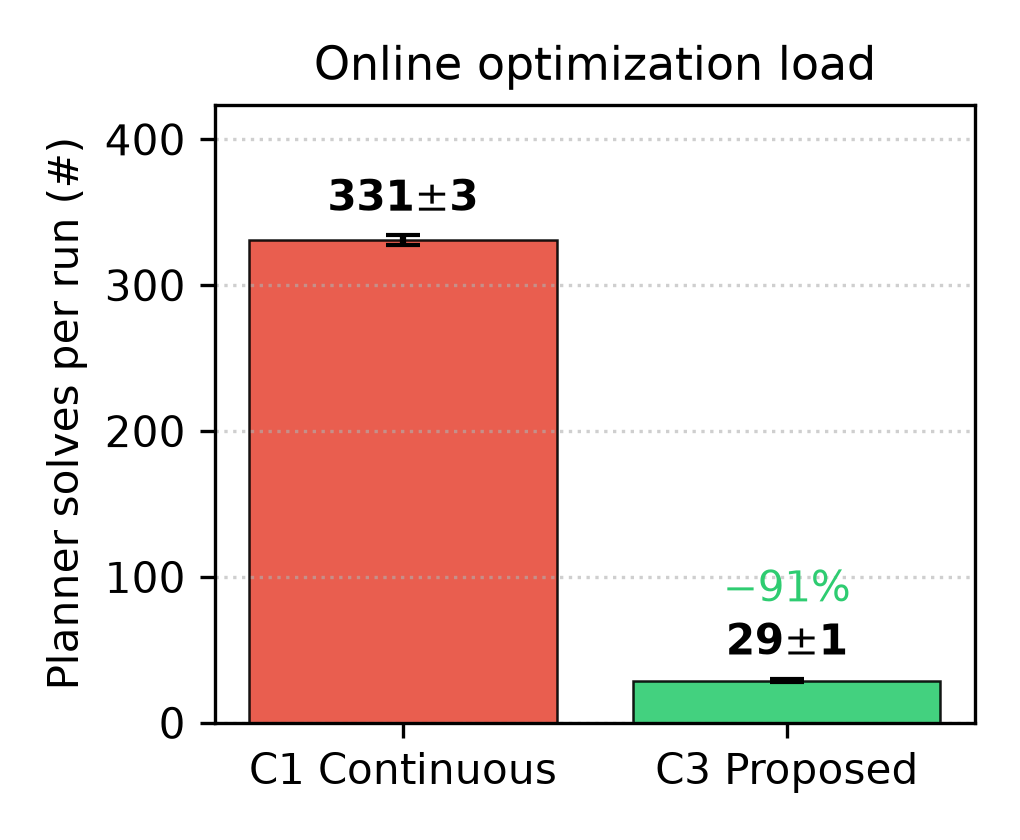
\includegraphics[width=0.82\columnwidth]{Figure_Solves.png}
\caption{Online planner solves per $40$\,s run (mean$\pm$std, $8$ runs/method):
continuous replanning (C1) vs.\ the perception-driven event trigger (C3), an
$\approx\!11\times$ ($91\%$) reduction at statistically equal tracking error.}
\label{fig:solves}
\end{figure}

We are explicit about what the occlusion experiment does \emph{not} show: when the
EKF ArUco updates are suppressed, the covariance grows the same way for both
configurations (peak $\tr\Sigma\approx0.17$ in the injected window for C1 and C3
alike; Fig.~\ref{fig:timeseries}), because the injected loss is independent of the
UAV's replanning strategy. Both recover once the measurement returns. Thus the
occlusion scenario demonstrates that the stress is real and the estimate stays
bounded and recovers, but it does \emph{not} evidence a covariance advantage for
C3 --- the demonstrated benefit of the event trigger is computational. The larger
full-run peak $\tr\Sigma$ in Table~\ref{tab:results} ($0.245$/$0.197$) is dominated
by the initial EKF-convergence/takeoff transient rather than the occlusion, and it
carries a large run-to-run standard deviation ($\pm0.16$); we therefore report the
occlusion-window peak, which isolates the injected-occlusion response and is
tightly repeatable, as the covariance metric of record.

\begin{table}[h]
\caption{Metrics from fresh simulation runs (mean\,$\pm$\,std over $R{=}4$ repeats
$\times$ \{nominal, occlusion\}$=8$ runs/method). Auto-generated into
\texttt{results/Table\_1\_Summary.csv} (table and prose share one window).
$^{\dagger}$Steady-state window $t\!\ge\!8$\,s (excludes the takeoff/EKF-convergence
transient). $^{\ddagger}$Full-run peak is dominated by that initial transient; the
occlusion-window peak isolates the injected-occlusion response and carries the
``both remain bounded'' point.}
\label{tab:results}
\begin{center}
\footnotesize
\begin{tabular}{|l|c|c|}
\hline
\textbf{Metric} & \textbf{C1 (Continuous)} & \textbf{C3 (Event-Trig.)}\\
\hline
Planner solves (\#) & \RESsolvesCone & \RESsolvesCthree\\
\hline
Mean tracking error (m)$^{\dagger}$ & \RESerrCone & \RESerrCthree\\
\hline
Mean $\tr\Sigma^{\dagger}$ & \REScovCone & \REScovCthree\\
\hline
Peak $\tr\Sigma$ (full run)$^{\ddagger}$ & \RESpeakfullCone & \RESpeakfullCthree\\
\hline
Peak $\tr\Sigma$ (occlusion window) & \RESpeakCone & \RESpeakCthree\\
\hline
Mean UAV solve time (ms) & \RESaruCone & \RESaruCthree\\
\hline
\end{tabular}
\end{center}
\end{table}

\begin{figure}[thpb]
\centering
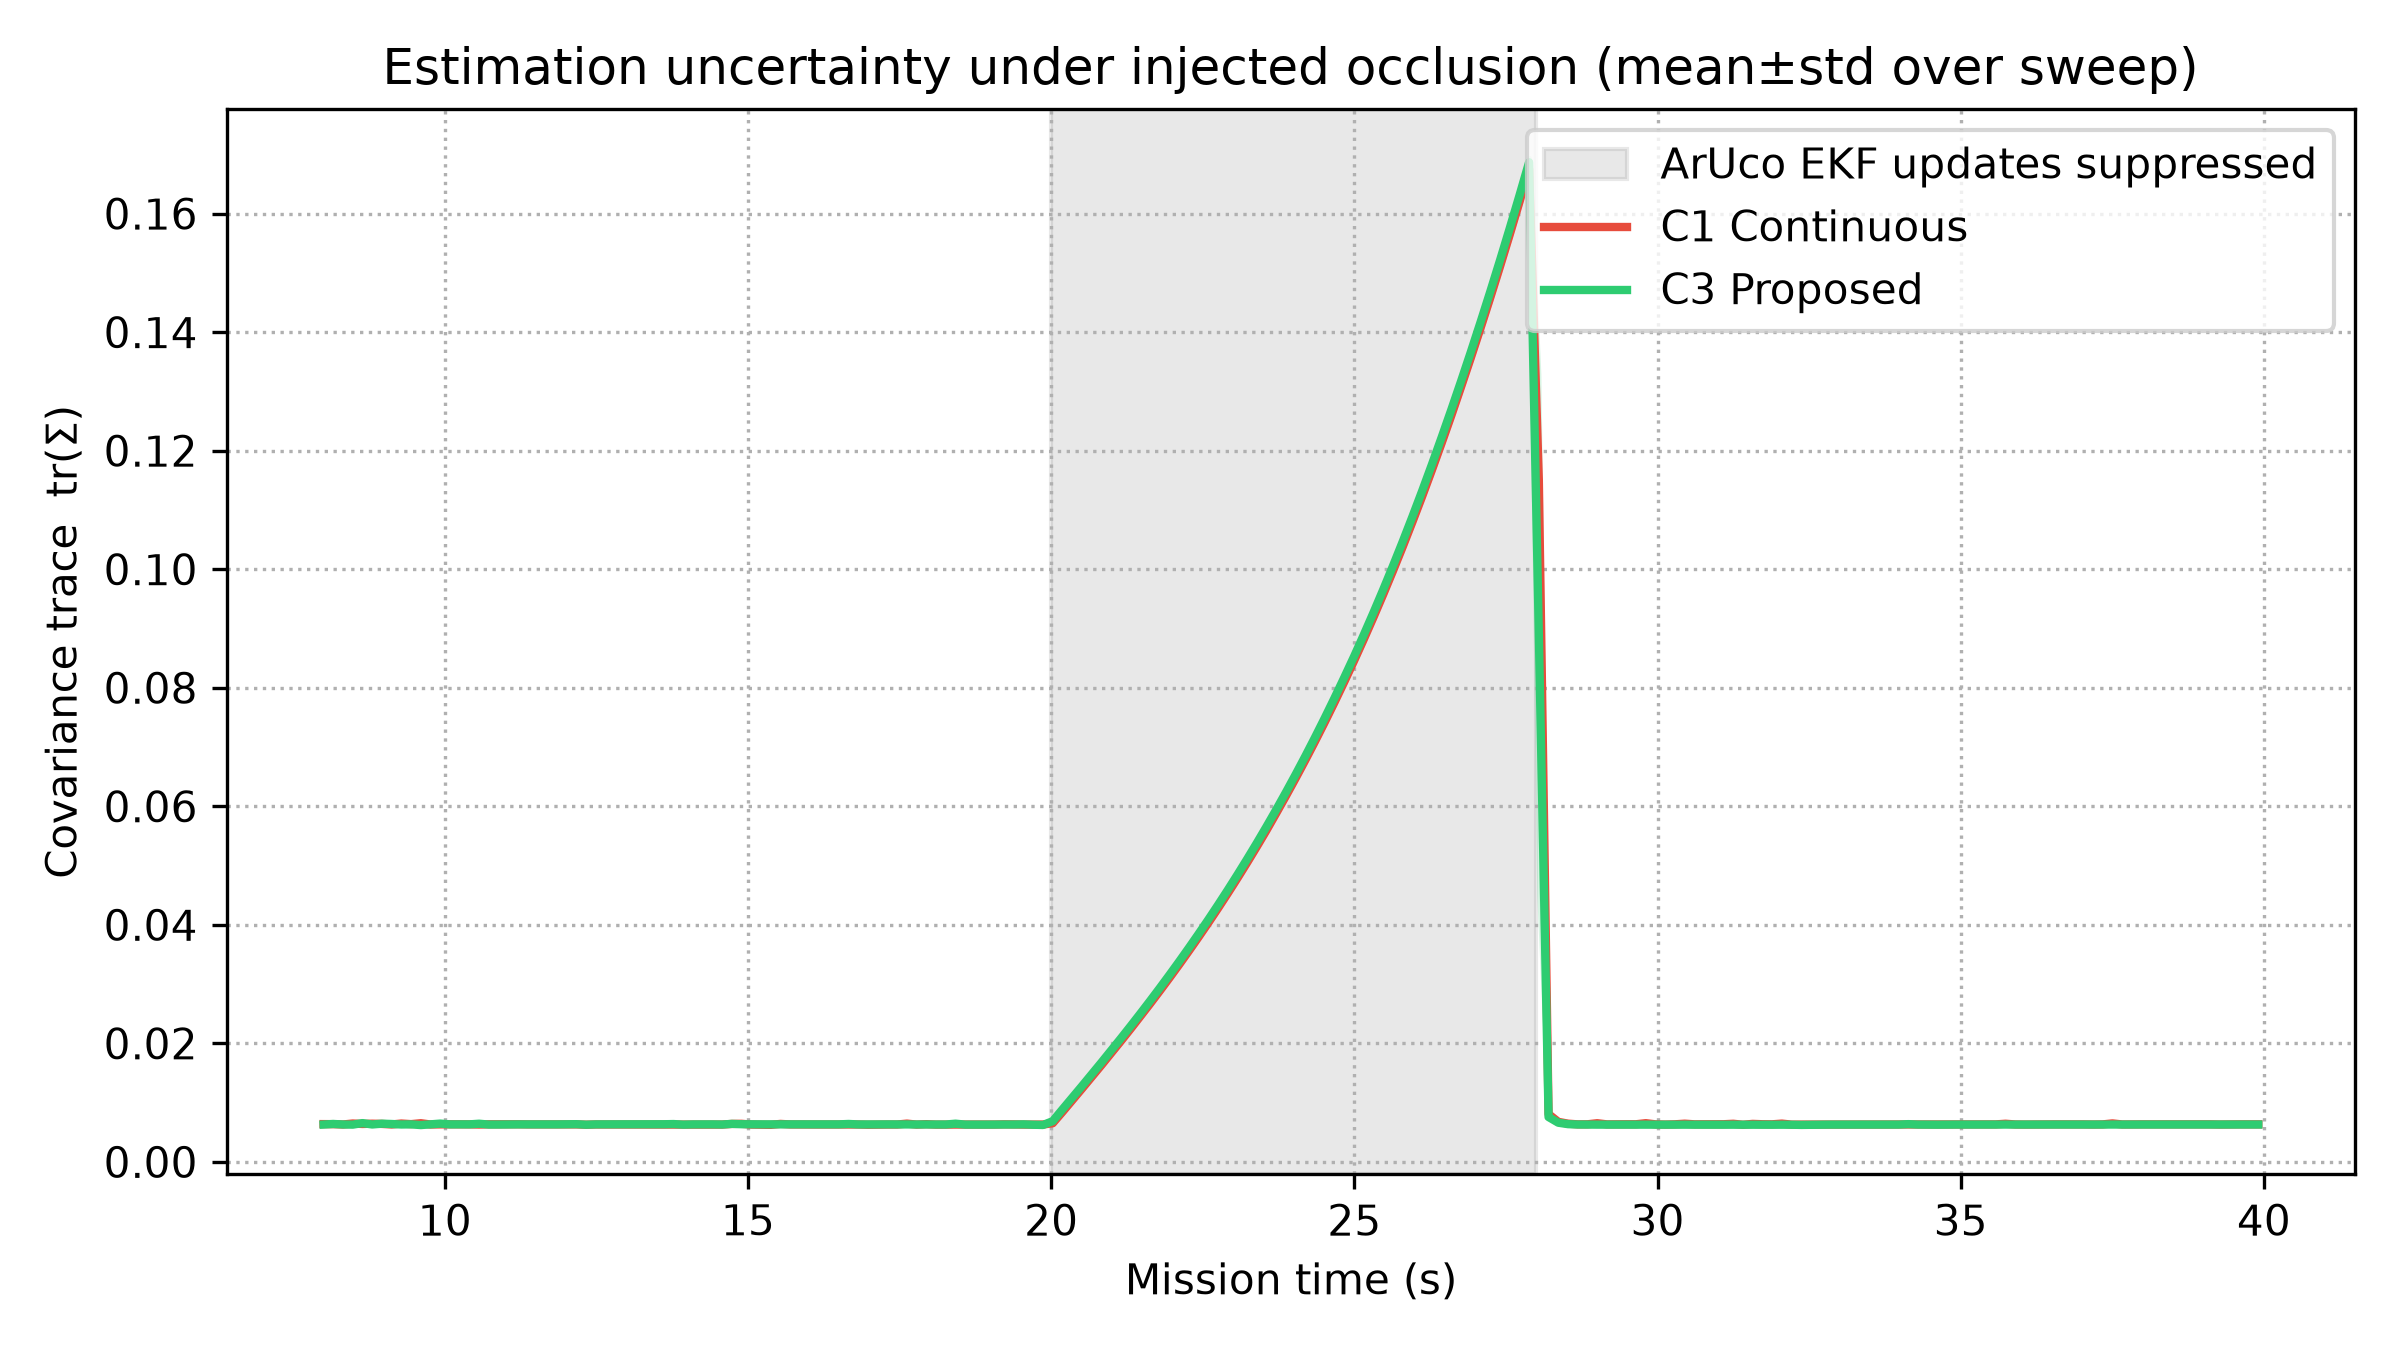
\includegraphics[width=0.95\columnwidth]{Figure_CovTrace.png}
\caption{Estimation uncertainty $\tr\Sigma(t)$ under injected occlusion (ArUco EKF
updates suppressed over the shaded window), mean$\pm$std over $R{=}4$ repeats, after
the takeoff transient. Both C1 (continuous) and C3 (event-triggered) exhibit the
same covariance growth and recovery: the injected loss is independent of the
replanning strategy. The event trigger's advantage is the $11\times$ reduction in
solve count (Table~\ref{tab:results}), not occlusion robustness.}
\label{fig:timeseries}
\end{figure}

\section{CONCLUSIONS}

We presented an observability-driven, event-triggered tube-MPC design for
aerial--ground tracking and a full SITL integration in ROS\,2/Gazebo. Our
validated result is computational: the perception-driven trigger reduces online
planner solves by $\approx\!11\times$ at statistically equal tracking accuracy over
$8$ paired runs. We are deliberate that this is the \emph{demonstrated} payoff --- the
trigger is observability-aware by design, but its isolated observability benefit is
not established on the present platform, because the UAV tracks tightly enough that
the FoV margin is not stressed and the tighter-FoV regime that would stress it is
not trajectory-reproducible under the current non-lockstep simulator. Future work:
a controllable-lag regime and a deterministic lockstep simulator to test the
observability claim; and, on the theory side, wiring the offline mRPI online, a
homothetic tube with recursive-feasibility guarantees, a $\sigma$-polytopic
fractional trigger, and hardware validation.

%%%%%%%%%%%%%%%%%%%%%%%%%%%%%%%%%%%%%%%%%%%%%%%%%%%%%%%%%%%%%%%%%%%%%%%%%%%%%%%%

\begin{thebibliography}{99}

\bibitem{mayne2005robust} D. Q. Mayne, M. M. Seron, and S. V. Rakovi\'c,
``Robust model predictive control of constrained linear systems with bounded
disturbances,'' \emph{Automatica}, vol.~41, no.~2, pp.~219--224, 2005.

\bibitem{mRPI} S. V. Rakovic, E. C. Kerrigan, K. I. Kouramas, and D. Q. Mayne,
``Invariant approximations of the minimal robust positively invariant set,''
\emph{IEEE Trans. Autom. Control}, vol.~50, no.~3, pp.~406--410, 2005.

\bibitem{mayne2000constrained} D. Q. Mayne, J. B. Rawlings, C. V. Rao, and
P. O. M. Scokaert, ``Constrained model predictive control: Stability and
optimality,'' \emph{Automatica}, vol.~36, no.~6, pp.~789--814, 2000.

\bibitem{falanga2018pampc} D. Falanga, P. Foehn, P. Lu, and D. Scaramuzza,
``PAMPC: Perception-aware model predictive control for quadrotors,'' in
\emph{IEEE/RSJ Int. Conf. Intelligent Robots and Systems (IROS)}, 2018.

\bibitem{platt2010belief} R. Platt, R. Tedrake, L. Kaelbling, and
T. Lozano-P\'erez, ``Belief space planning assuming maximum likelihood
observations,'' in \emph{Robotics: Science and Systems (RSS)}, 2010.

\bibitem{vandenberg2012motion} J. van den Berg, S. Patil, and R. Alterovitz,
``Motion planning under uncertainty using iterative local optimization in belief
space,'' \emph{Int. J. Robotics Research}, vol.~31, no.~11, pp.~1263--1278, 2012.

\bibitem{eqtami2010event} A. Eqtami, D. V. Dimarogonas, and K. J. Kyriakopoulos,
``Event-triggered control for discrete-time systems,'' in \emph{American Control
Conference (ACC)}, 2010, pp.~4719--4724.

\end{thebibliography}


\end{document}
